\begin{infocard}{Funciones}
    \begin{minipage}{0.3\textwidth}
        \begin{figure}[H]
            \centering
            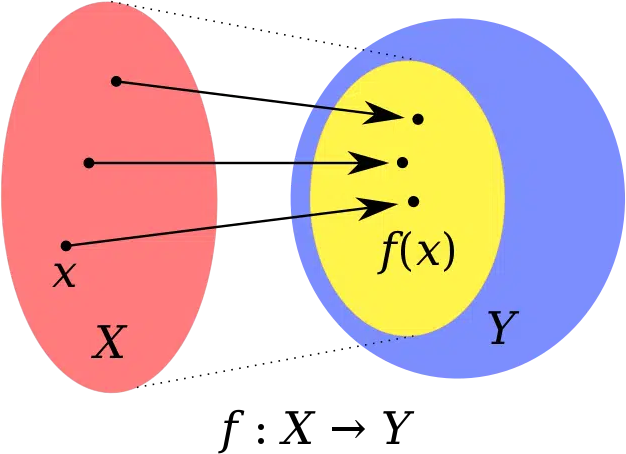
\includegraphics[width=0.6\linewidth]{../images/Rango-de-una-funcion}
            \caption{}
            \label{fig:funciones}
        \end{figure}
    \end{minipage}\hfill
    \begin{minipage}{0.65\textwidth}
        Considerando dos conjuntos de números, $A$ y $B$, una función asocia a cada elemento
        $x$ del conjunto $A$ (valor de entrada) un único elemento y del conjunto $B$ (valor de
        salida) mediante una regla de correspondencia $f$.\\

        El número $x$ que pertenece a un conjunto $A$ es la variable independiente. El número
        $y$ asociado con el valor $x$ por la regla de correspondencia $f$ es la variable
        dependiente.
        % La regla de correspondencia, que puede ser una expresión algebraica, se acostumbra denotar con alguna letra del alfabeto y la variable dependiente entre paréntesis, por ejemplo $f(x)$ y se lee \emph{efe de equis}. La expresión algebraica de una función
        % es una identidad que permite obtener el valor de y cuando se sabe el valor de $x$, realizando operaciones algebraicas. Es una manera de obtener los valores de la variable
        % independiente sin tener que recurrir a la gráfica de la expresión algebraica.
        % Por ejemplo, la función $f(x) = 2x + 3$ asocia a cada valor de la variable independiente $x$, un valor de la variable dependiente $y$ con la regla de correspondencia: multiplicar
        % el valor de entrada por 2 y luego sumar 3. Se puede escribir también $y = 2x + 3$.
    \end{minipage}
\end{infocard}